\documentclass[tikz,border=2pt]{standalone}
\usetikzlibrary{arrows.meta,positioning,calc,fit,backgrounds}
\usepackage{fontspec}
\setmainfont{TeX Gyre Termes}
\setsansfont{Roboto}
\begin{document}
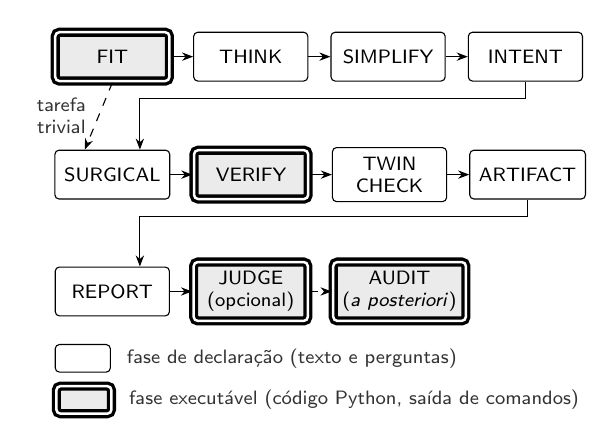
\begin{tikzpicture}[
  font=\sffamily\scriptsize,
  >={Stealth[length=4pt]},
  fase/.style={draw, thin, rounded corners=1.5pt, minimum width=1.45cm, minimum height=0.62cm, align=center, fill=white},
  exec/.style={fase, very thick, double distance=0.9pt, fill=black!8},
  nota/.style={font=\sffamily\scriptsize, align=center, text=black!80}
]
% linha 1
\node[exec] (fit) {FIT};
\node[fase, right=0.28cm of fit] (think) {THINK};
\node[fase, right=0.28cm of think] (simp) {SIMPLIFY};
\node[fase, right=0.28cm of simp] (intent) {INTENT};
% linha 2
\node[fase, below=0.85cm of fit] (surg) {SURGICAL};
\node[exec, right=0.28cm of surg] (verify) {VERIFY};
\node[fase, right=0.28cm of verify] (twin) {TWIN\\CHECK};
\node[fase, right=0.28cm of twin] (art) {ARTIFACT};
% linha 3
\node[fase, below=0.85cm of surg] (rep) {REPORT};
\node[exec, right=0.28cm of rep] (judge) {JUDGE\\(opcional)};
\node[exec, right=0.28cm of judge] (audit) {AUDIT\\(\textit{a posteriori})};
% setas
\draw[->] (fit) -- (think);
\draw[->] (think) -- (simp);
\draw[->] (simp) -- (intent);
\draw[->] (intent.south) -- ++(0,-0.22) -| ($(surg.north)+(0.35,0)$);
\draw[->] (surg) -- (verify);
\draw[->] (verify) -- (twin);
\draw[->] (twin) -- (art);
\draw[->] (art.south) -- ++(0,-0.22) -| ($(rep.north)+(0.35,0)$);
\draw[->] (rep) -- (judge);
\draw[->, dashed] (judge) -- (audit);
% atalho trivial
\draw[->, dashed] (fit.south) -- node[left, nota, xshift=-1pt] {tarefa\\trivial} ($(surg.north)-(0.35,0)$);
% rotulos de legenda
\node[fase, anchor=north west, minimum width=0.7cm, minimum height=0.35cm] (l1) at ($(rep.south west)+(0,-0.35)$) {};
\node[nota, right=0.08cm of l1, anchor=west] {fase de declaração (texto e perguntas)};
\node[exec, anchor=north west, minimum width=0.7cm, minimum height=0.35cm] (l2) at ($(l1.south west)+(0,-0.15)$) {};
\node[nota, right=0.08cm of l2, anchor=west] {fase executável (código Python, saída de comandos)};
\end{tikzpicture}
\end{document}
